\documentclass{beamer}

\usepackage{polyglossia}
\setdefaultlanguage[spelling=new, babelshorthands=true]{german}

\usepackage{amssymb}
\usepackage{pifont}
\usepackage{graphicx}
\usepackage{verbatim}
\usepackage{default}

\newcommand{\cmark}{\ding{51}}
\newcommand{\xmark}{\ding{55}}

\title{Mitrax}
\author{Benjamin Buch}
\date{11. Oktober 2016}

\begin{document}
\begin{frame}
    \frametitle{Kernverbesserungen von Mitrax}
    \begin{itemize}
        \item Eigener Datentyp für Zeilen und Spalten
        \item Elementrepräsentationsunabhängige Schnittstelle
        \begin{itemize}
            \item Leicht erweiterbar für neue Arten der Datenrepräsentation (Adapter, Views, GPU …)
        \end{itemize}
        \item Intuitive und sichere Initialisierungssyntax
        \item „Zero-Overhead“ – Compiler kann bestmöglich optimieren
        \item Support von \texttt{constexpr}
    \end{itemize}
\end{frame}
\begin{frame}
    \frametitle{Was macht eine Matrix aus?}
    \begin{itemize}
        \item Anzahl Zeilen und Spalten; bekannt zur:
        \begin{itemize}
            \item Compilezeit (Mitrax, Eigen, Boost.uBLAS)
            \item Laufzeit (Mitrax, Eigen)
        \end{itemize}
        \item Entsprechend rechteckig angeordnete Elemente gleichen Typs
        \begin{itemize}
            \item Existieren im Speicher (Mitrax, Eigen, Boost.uBLAS)
            \item Zur Compilezeit bekannt (Mitrax)
            \item Erzeugung bei Zugriff (Mitrax)
        \end{itemize}
    \end{itemize}
\end{frame}
\begin{frame}
    \frametitle{Bereitstellung der Elemente einer Matrix}
    \begin{itemize}
        \item \textbf{constexpr}; Elemente sind zur Compilezeit bekannt und können direkt für Berechnungen verwendet werden. (Mitrax)
        \item \textbf{Stack} (Mitrax, Eigen)
        \item \textbf{Heap} (Mitrax, Eigen, Boost.uBLAS)
        \item \textbf{View}; Das Matrix-Objekt besitzt die Daten nicht selbst, sondern ermöglicht nur den Zugriff. (zukünftig Mitrax)
        \item \textbf{Adapter}; Es wird ein anderer Datentyp (z. B. Eigen::Matrix) verwendet (Mitrax)
        \item \textbf{Funktion}; Beim Zugriff wird der Wert eines Elementes entsprechend seiner Position in der Matrix und einer gegebenen Berechungsvorschrift berechnet. (zukünftig Mitrax)
        \item \textbf{GPU-Speicher} (zukünftig Mitrax, teilweise Eigen)
        \item \textbf{anderer Speicher}; Festplatte, FPGA … (zukünftig Mitrax)
    \end{itemize}
\end{frame}
\begin{frame}
    \frametitle{Typisierte Zeilen \& Spalten}
    \begin{itemize}
        \item Eigener Typ für Zeilen und Spalten \\
            \hspace{1em}\texttt{struct col\_t< 4 >} \\
            \hspace{1em}\texttt{struct row\_t< 7 >}
        \item User-defined literals \\
        \hspace{1em}\texttt{4\_C} \\
        \hspace{1em}\texttt{7\_R}
        \item Typsicheres Rechnen mit Dimensionen \\
        \hspace{1em}\texttt{4\_C + 3\_C \cmark} \\
        \hspace{1em}\texttt{7\_R + 2\_C \xmark}
    \end{itemize}
\end{frame}
\begin{frame}[fragile]
    \frametitle{Intuitive \& sichere Initialisierung}
    \begin{itemize}
        \item Anforderungen:
        \begin{itemize}
            \item Alle Elemente haben nach der Initialisierung einen definierten Wert
            \item Direkte Initialisierung für kleine Matritzen
        \end{itemize}
    \item Umsetzung:
    \begin{itemize}
        \item Initialisierung mit Default-Value
\begin{verbatim}
auto matrix = make_matrix_v(3_C, 2_R, 3.f);
\end{verbatim}
        \item Direkte elementweise Initialisierung
\begin{verbatim}
auto matrix = make_matrix(3_C, 2_R, {
    {1, 2, 3},
    {4, 5, 6}
});
\end{verbatim}
\end{itemize}
\end{itemize}
\end{frame}
\begin{frame}
    \frametitle{Anwendung: \texttt{constexpr} Matrix (1)}
    \begin{itemize}
        \item Beim Sobel-Operator sind Dimensionen und Elemente der Faltungsmatrix zur Compilezeit bekannt
        \item Anmerkungen zum folgenden Benchmark:
        \begin{itemize}
            \item Die Faltungsoperation ist für Mitrax, Boost.uBLAS und Eigen identisch implementiert
            \item Die Bildmatrix liegt immer auf dem Heap und hat Laufzeit-Dimensionen
            \item Bei der Faltungsmatrix richtet sich dies nach der verwendeten Bibliothek:
            \begin{itemize}
                \item Mitrax: Compilezeit-Dimensionen, Daten sind constexpr
                \item Eigen: Compilezeit-Dimensionen, Daten auf dem Stack
                \item Boost.uBLAS: Laufzeit-Dimensionen, Daten auf dem Heap
            \end{itemize}
        \end{itemize}
    \end{itemize}
\end{frame}
\begin{frame}
    \frametitle{Anwendung: \texttt{constexpr} Matrix (2)}
    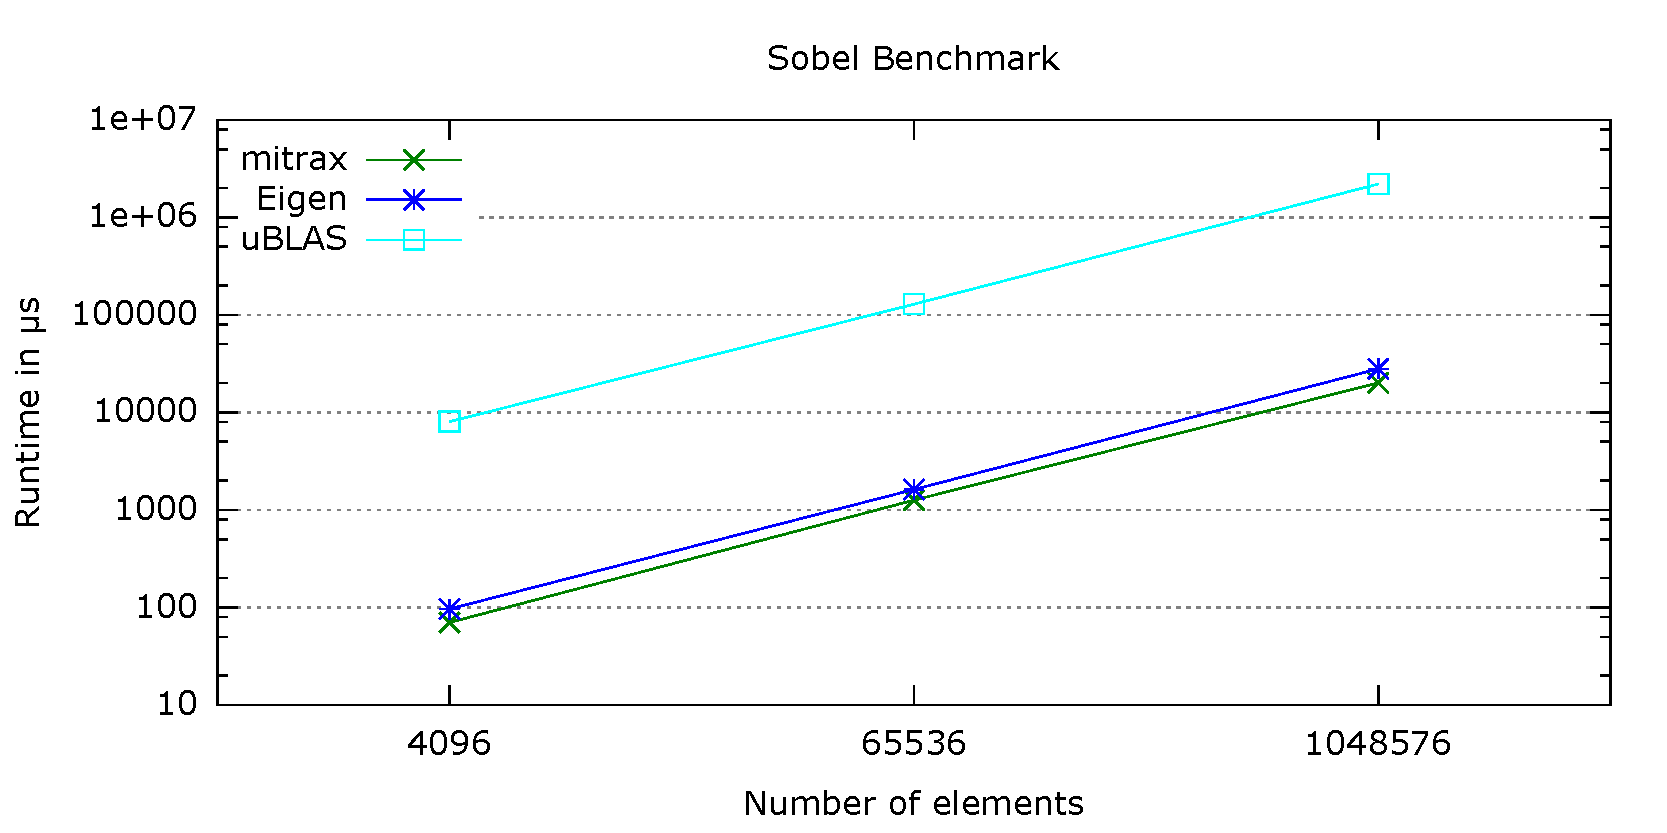
\includegraphics[width=\textwidth]{images/sobel2.pdf}
\end{frame}
\begin{frame}[fragile]
    \frametitle{Vektoren sind Matritzen}
    \begin{itemize}
        \item Falls Zeilen oder Spalten zur Compilezeit den Wert 1 haben, werden durch die Schnittstelle zusätzliche Funktionen angeboten, ohne dass sich die Implementierung darum kümmern muss
        \begin{itemize}
            \item Zugriffsoperator für Vektoren:
\begin{verbatim}
auto vector = make_matrix(1_C, 3_R, {{1}, {2}, {3}});
vector(0, 2) = 7; // normaler Matrix-Zugriff
vector[2] = 5;    // vereinfachter Vektor-Zugriff
\end{verbatim}
            \item Vereinfachte Erstellung:
\begin{verbatim}
auto vector = make_col_vector(3_R, {1, 2, 3});
\end{verbatim}
        \end{itemize}
    \end{itemize}
\end{frame}
\end{document}
